\chapter{\chapterFour}
\label{chp:4}

\textit{This chapter contains our proposed system to achieved our goals which explained in Chapter 1. First, assumptions, requirements and steps to achieve thesis' main goal. on our system are presented. The chapter continues with reasonings on our chosen embedded platform, Arduino. Then, the selected error correcting code which will be used in the system is explained. Afterwards, we present our data and key storage scheme and also our way to generate key using SRAM PUF. Last, our idea to use bits locations as a PUF challenge is shown. }

\section{Assumptions, Requirements and Steps To Achieve Main Goal}\label{ch:use_case}

% As mentioned in the first chapter, a subset of this thesis goal is to provide a secure data protection and key storage scheme using SRAM PUF. This thesis goal describes the use case of our proposed system.
To focus the thesis approach, we have defined several assumptions. First, the field of the constructed SRAM PUF application is decided to be only available offline. Accessing the SRAM PUF requires the user to have the device next to his/her side. Second, an attacker cannot access the SRAM directly. An attacker may gain the knowledge of the helper data and challenge used in the PUF concept. Last, there is no analysis and/or solution against physical attacks, e.g side channel attacks, in our secure data and key storage scheme. The scheme is designed to be secure against theoretical attacks.

We also have define a set of requirements related to our system. Below are the requirements defined:

\begin{enumerate}
    \item Software-based construction\newline
    There should be no major hardware modification or hardware design to implement the project.
    \item Patent/license free\newline
    Any dependent component of the design should be in public domain.
    \item Open-source and collaboration oriented\newline
    If there's a reliable open source project which can be a foundation for this thesis project, instead of building our own software, it is preferred to use that project. This will significantly reduce the time consumed on constructing the whole project. Using other project source code can also increase the collaboration atmosphere. In addition, this requirement may help this project to be known by others since they might introduce our project as one of the projects that uses their code.
    \item Key-length security level\newline
    The goal on the key-length security level is 256-bits. The concept constructed should be able to use this level and the project's security should be uncompromised even though the key-length is only 256-bits.
    \item Off-the-shelf SRAM\newline
    The SRAM involved in the thesis should be easily available in the market and cost insignificant.
    \item Affordable\newline
    The total hardware required to produce the system should be inexpensive.
    \item Reproducible\newline
    Anyone should be able to reproduce this thesis experiment with no significant effort.
\end{enumerate}

Another thing that we would like to address is steps required to achieve this thesis' main goal which related to answering this thesis' problem statement. As shown in Section \ref{ch:problem}, the problem statement is "\problemStatement".
Below are several steps expected to be done as an attempt to achieve this goal:
\begin{enumerate}
  \item Choose embedded platform on where the system will be built.
  \item Select a type of error-correcting codes which will be used as an element in the key generation scheme. The memory required by the error correcting codes has to fit in the embedded platform's internal memory.
  \item Search and analyze existing SRAM PUF-based key generation schemes. Propose one of them to be used as the key generation procedure in this thesis and also calculate the maximum error rate that can be handled by the key generation scheme.
  \item Propose and construct a system to enable secure data and key storage based on the selected key generation scheme and SRAM PUF technology. Any library required in the system has to be open-source. In addition, the constructed system has to work without any explicit hardware design, in other words, \textit{software-based} construction.
  \item Get off-the-shelf SRAM components available in the market.
  \item Locate the stable bits inside each SRAM using bit selection algorithm.
  \item Test the reliability of SRAM's stable bits. The error rate of the stable bits (referred as HD\textsubscript{intra}) has to be lower than the maximum error rate that can be handled by the key generation scheme.
  \item If the SRAM's stable bits is reliable, continue using this SRAM as the root-of-trust in the proposed secure data and key storage.
  \item Test the complete secure data and key storage scheme in various scenarios.
\end{enumerate}

\section{Arduino Mega 2560 as the Embedded Platform}

One of the important details of our system is choosing the platform on where the system will be built.
There are two major candidates, Arduino and Raspberry Pi. Both are chosen due to its popularity, availability (easy to get), and various types available. High popularity means the debugging process can be done fast and many references are available online to help the system development. Availability is important because this thesis goal should be easily used by anyone. Low availability will reduce significantly reusability of this project and user's interest. Various types available is a good option for system flexibility. For example, if a user wants to develop a more complex system on top of this thesis' system or desire to use a more complex error correcting codes, he/she can choose a platform with higher computing capability.
Besides those three factors, another feature which lead on selecting Raspberry Pi and Arduino is their GPIO. GPIO availability will enable easy communication between the SRAM and the embedded platform.

Compared to Arduino, Raspberry Pi offers a higher computing capability and relatively easier development. This is because Raspberry Pi is basically a mini Linux computer. One can develop a software using C, C++, Python, etc. in Raspberry Pi which may fasten the project development, especially for a developer who already familiar with a specific programming language. Unfortunately, Raspberry Pi requires a longer startup time compared to Arduino. It also requires higher electrical power. If one wants to use the developed project in the embedded area, this two factor is a major trade-off.

Due to the above consideration, Arduino is chosen. Even though one has to construct the system in C++, this can be a positive thing since one can maximize the computing capability easily. Moreover, Arduino itself is an open-source project which enable anyone to develop their own boards and software libraries \cite{arduino}.

There are various Arduino types available on the market. The chosen Arduino type is Arduino Mega 2560. It is selected because it offers larger memory capability compared to other types, such as 256k bytes of Flash memory, 8k bytes internal SRAM, and 4k byte EEPROM.
Besides, it also has 54 digital I/O pins and 16 analog I/O pins which ease the communication to external SRAM.

\section{BCH Codes as Error Correcting Codes}
As shown in previous chapter, there are two major categories in ECC; soft-decision and hard-decision code. We choose to use hard-decision ECC over the soft decision one since there is no requirement to provide the error probability function on SRAM cells. Futhermore, between two examples of hard-decision ECC, we particularly pick BCH codes as the ECC due to lower computing resource required compared to Reed-Solomon Codes. BCH also better at correcting random errors than Reed-Solomon Codes.

As mentioned in the previous chapter, BCH codes are flexible Error Correcting Codes (ECC) shown by multiple parameters available. The only fixed parameter is $q$ since the problem is in binary form ($q=2$). The source code for BCH codes utilized in our construction is a modified version of Robert Morelos-Zaragoza's version which can be retrieved at \cite{bch_code}. This code is selected because it can support $m$ ranging from 2-20 which mean the length of the code that can be corrected ranging from 2 until 1048575. When using BCH codes, one should be careful on deciding the parameters that will be used, for example, larger $m$ or $n$ means a bigger memory needed.
These parameters should be determined with several considerations, such as the inner hamming distance of SRAMs and memory available on Arduino Mega 2560.

On deciding the value $m$, a further look on the memory required during the error correction computation need to be done. Inside the bch codes from \cite{bch_code}, the decoding method requires the largest memory compared to other procedures. There are six parameters that depend on $m$ which are $elp$, $d$, $l$, $u_lu$, $s$, and $err$. Table \ref{tab:memorybch} shows the required memory given the $m$ value.

\begin{table}[htbp]
  \centering
  \caption{Memory required (bytes) given the value of $m$.}
    \begin{tabular}{|l|l|l|l|}
    \hline
    \multicolumn{1}{|c|}{\textbf{m}} & \multicolumn{1}{c|}{\textbf{Bytes Required}} & \multicolumn{1}{c|}{\textbf{m}} & \multicolumn{1}{c|}{\textbf{Bytes Required}} \\
    \hline
    2     & 53    & 12    & 16805897 \\
    \hline
    3     & 129   & 13    & 67166217 \\
    \hline
    4     & 377   & 14    & 268550153 \\
    \hline
    5     & 1257  & 15    & 1073971209 \\
    \hline
    6     & 4553  & 16    & 4295426057 \\
    \hline
    7     & 17289 & 17    & 17180786697 \\
    \hline
    8     & 67337 & 18    & 68721311753 \\
    \hline
    9     & 265737 & 19    & 274881576969 \\
    \hline
    10    & 1055753 & 20    & 1099518967817 \\
    \hline
    11    & 4208649 &       &  \\
    \hline
    \end{tabular}%
  \label{tab:memorybch}%
\end{table}%

Since the internal SRAM in Arduino only has 8k bytes capacity, the chosen $m$ is 6 (requires 4553 bytes, around 55\% of total SRAM available in Arduino). This parameter will result in possible $n$ between 32 and 63. $n$ is chosen to be 63 to maximize the length code that can be encoded.
The combination of $m$ = 6 and $n$ = 63 results in various $k$ and $t$ that can be chosen. The combination of all parameter possible is shown on \ref{tab:bch}.

\begin{table}[htbp]
  \centering
  \caption{BCH parameter for $m$ = 6 and $n$ = 63.}
    \begin{tabular}{|r|r|}
    \hline
    \multicolumn{1}{|c|}{\textbf{k}} & \multicolumn{1}{c|}{\textbf{t}} \\
    \hline
    \multicolumn{1}{|l|}{57} & \multicolumn{1}{l|}{1} \\
    \hline
    51    & 2 \\
    \hline
    45    & 3 \\
    \hline
    39    & 4 \\
    \hline
    36    & 5 \\
    \hline
    30    & 6 \\
    \hline
    24    & 7 \\
    \hline
    18    & 10 \\
    \hline
    16    & 11 \\
    \hline
    10    & 13 \\
    \hline
    7     & 15 \\
    \hline
    \end{tabular}%
  \label{tab:bch}%
\end{table}%
To maximize the error correction capability, $k$ = 7 and $t$ = 15 is chosen. All these parameter combination will enable error correction capability 23.8\% of the data length. To summarize, here are the chosen parameters:
\begin{itemize}
\item $n$: 63
\item $k$: 7
\item $d$: 31
\item $t$: 15
\end{itemize}

\section{Data and Key Storage Scheme} \label{chp:data_protection_scheme}

Figure \ref{fig:scheme-data-protection} shows the scheme to protect user's data and key. On an attempt to protect the user's data and key, our proposal is divided into three major parts, first is generate the final key, and the rest is using the final key either to encrypt or decrypt data.
To prevent unauthorized person accessing the data with a stolen PUF, an idea from multi-factor authentication is utilized. Instead of just depending on the PUF device to access the key, a combination of PUF device and user knowledge is presented. User knowledge that used here is password.
User's password is combined with the PUF-generated key to generate a \textbf{final key} using HMAC. The input message to the HMAC is the user's password and the input key to the HMAC is the PUF-generated key. The HMAC function proposed to use is HMAC-SHA3 with key length 256 bits.
The final key can be used to encrypt and decrypt user data/key. To decrypt and encrypt the data, a symmetric encryption algorithm is preferred over the asymmetric one. The symmetric encryption algorithm used is AES with key length 256 bits.

\begin{figure}[tph!]
    \centerline{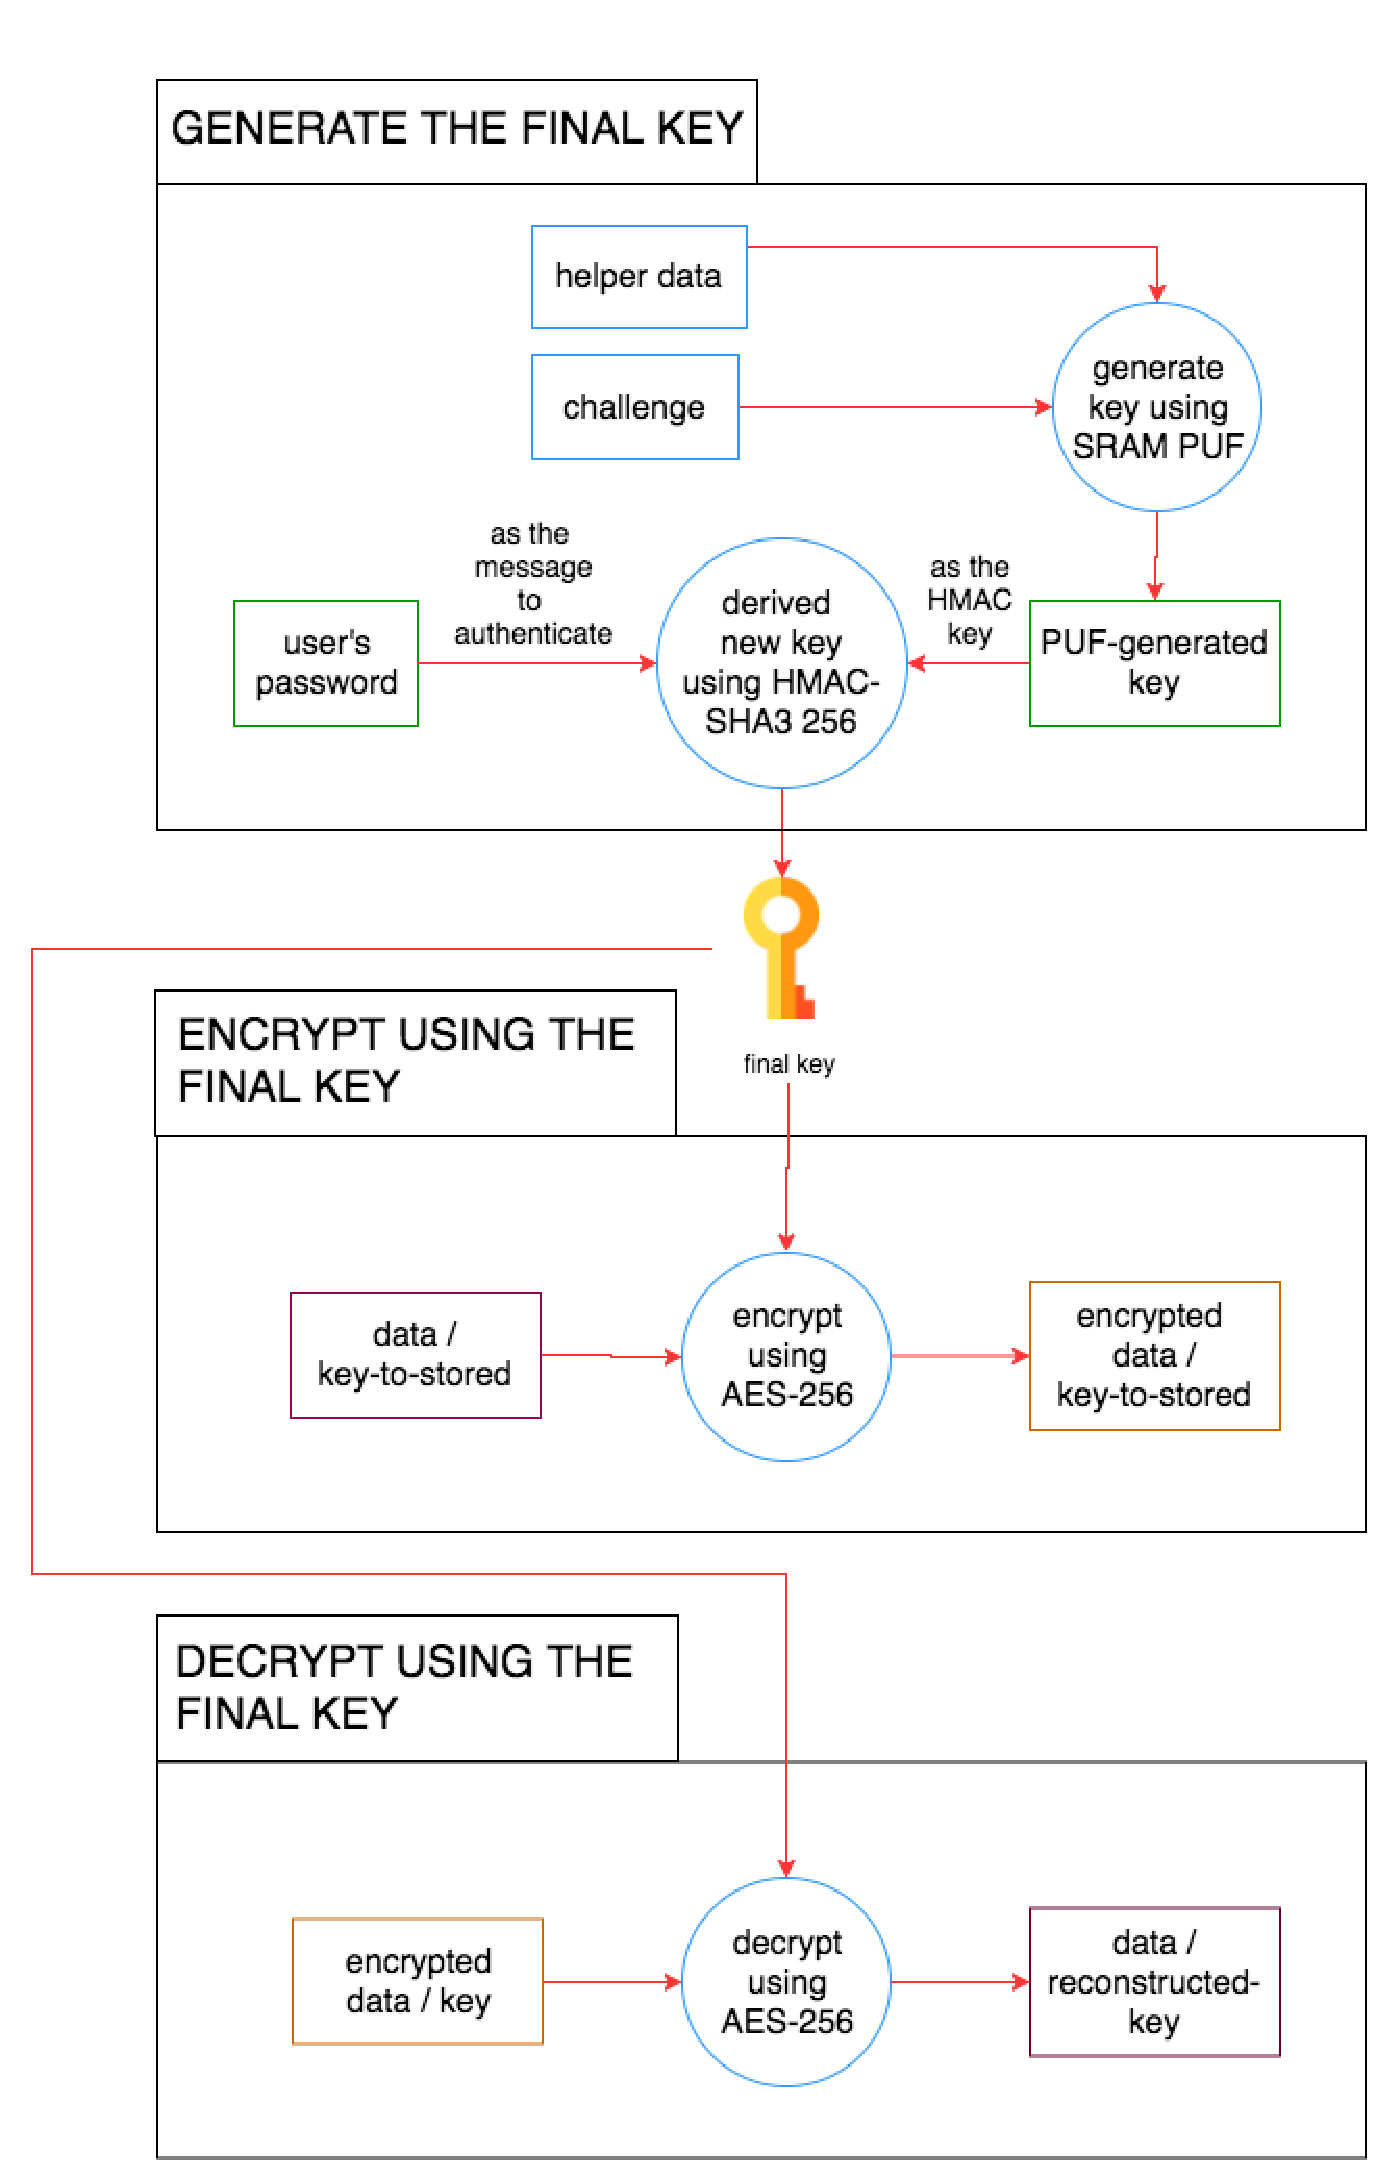
\includegraphics[width={0.9\textwidth}]{images/proposed}}
    \caption{Scheme for secure data and key storage. There are three stages in here; generate the final key, encrypt using the final key and decrypt also using the final key.}
    \label{fig:scheme-data-protection}
\end{figure}

% We believe this scheme is secure due to several assumption.
% First, if the attacker decides to attack the scheme by applying a cryptanalysis directly to the ciphertext, the attacker has to break the security level of AES-256. If brute-force attack is applied to AES-256, the attacker has to try all possibilities of $2^{256}$ keys which roughly equals to $1.157920892373163 \times 10^{77}$. Even if one can try ten thousands keys every second, the total time needed to try all combinations is still $3.67 \times 10^{65}$ years (longer than the age of the universe which is $14 \times 10^9$ years old).
% The attacker may also apply key-recovery attack using a technique called biclique attack \cite{10.1007/978-3-319-19962-7_3}. Even though this technique is the best known attack on AES-256, this technique still requires time complexity of $2^{254.27}$ and data complexity of $2^{40}$.

\section{Key Generation Scheme}

As shown in the previous section, the secure data and key storage scheme requires the PUF to generate the key which will be used to generate the final key. The key generation scheme used in this project is a modified version of Figure \ref{fig:cryptographic_key_generation} proposed in \cite{cryptographic_key_generation}. Instead of using $n$ = 255, the scheme used in this project will choose $n$ = 63. The parameter \textit{n, k, t, d} is similar to the parameter chosen in the previous section, BCH error correcting code. Figure \ref{fig:key-generation-scheme} illustrates the mentioned scheme.
Using this scheme, to generate a key with length 256-bits requires 37 blocks of this scheme, which lead to 2331 bits required. 37 blocks are calculated from $256\div7=36.57$, rounded-up resulting in 37. 7 comes from the key generated from 63 bits of data using this scheme. Since one block needs 63 bits of data, 37 blocks require $37\times63=2331$ bits.
In addition, if you look further into the scheme, there is an entropy loss as many as 7 bits every 63 bits input during the generation of helper data. Due to this entropy loss, this scheme can only correct errors on maximum 8 bits instead of 15 bits. Based on this reason, to ensure the key generation scheme always produced the same key, the SRAM component used as root-of-trust has to have maximum error rate (shown by HD\textsubscript{intra}) 12.7\% (calculated from $8\div63\times100\%$).

\begin{figure}[tph!]
    \centerline{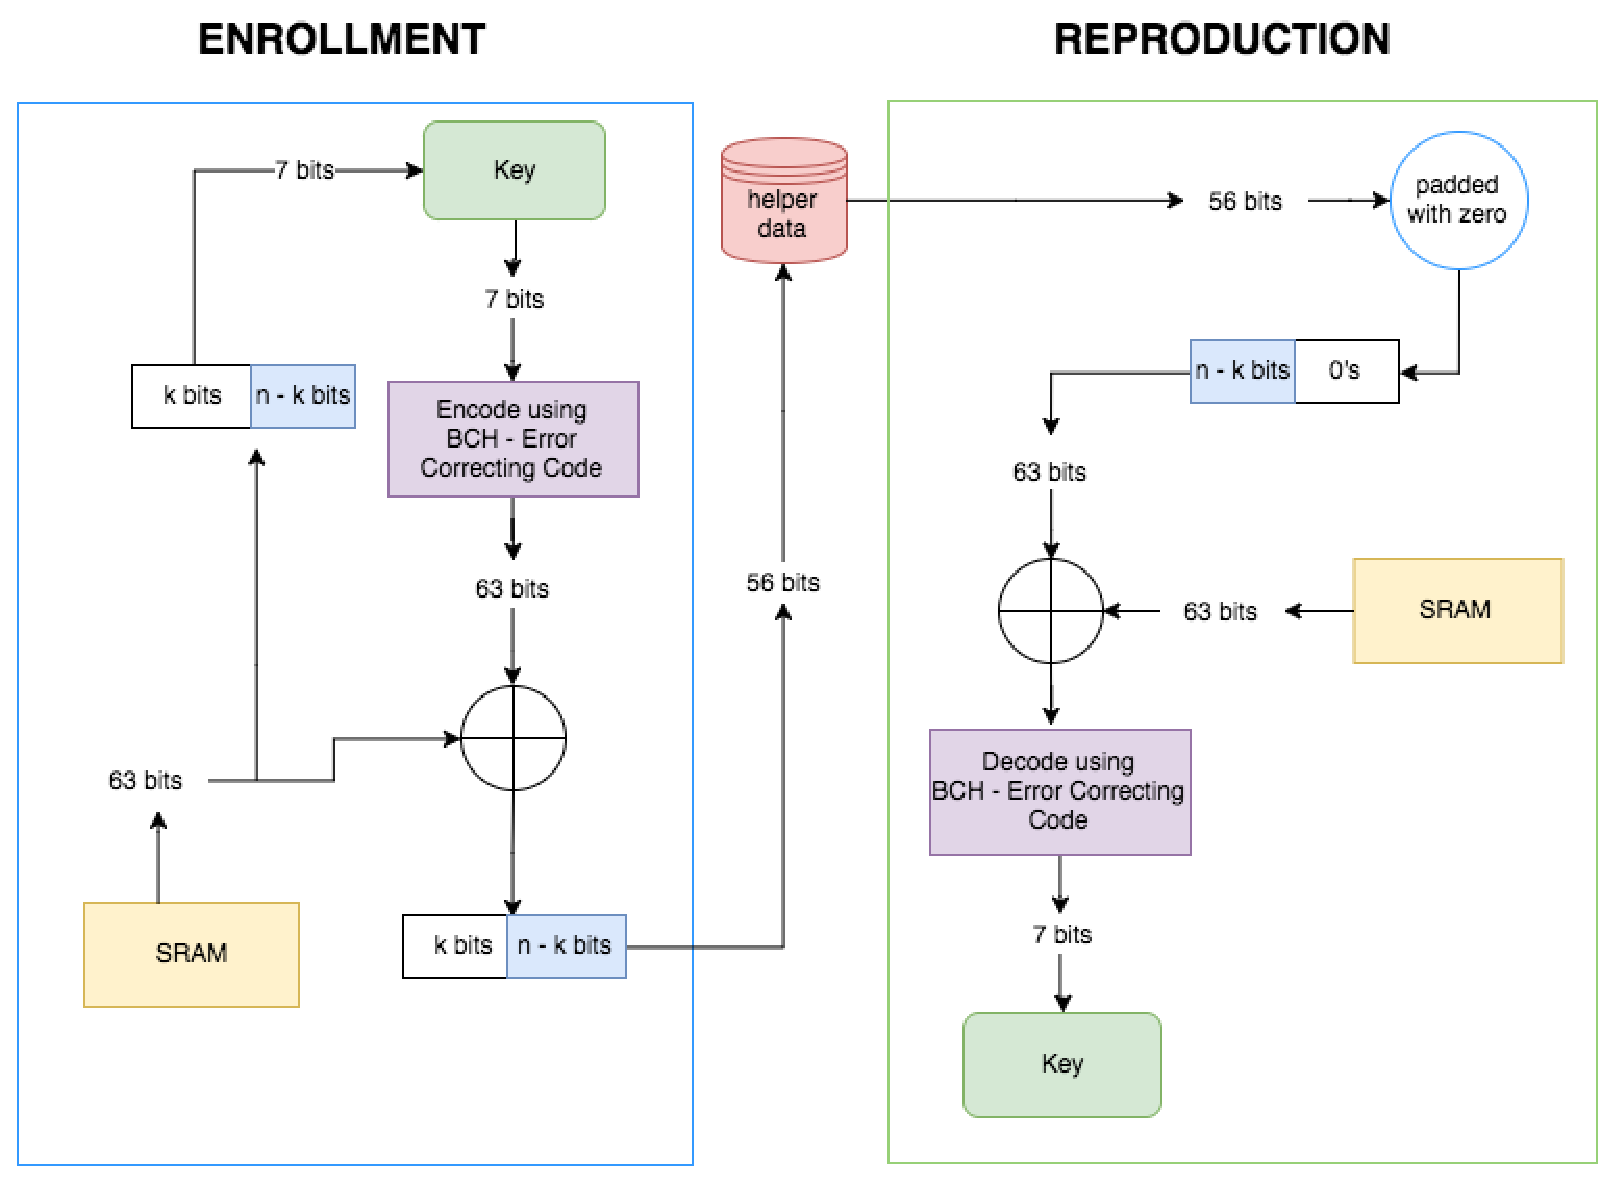
\includegraphics[width={\textwidth}]{images/key}}
    \caption{Scheme for key generation. $n$ = 63, $k$ = 7, $t$ = 15, $d$ = 31.}
    \label{fig:key-generation-scheme}
\end{figure}


\section{Bits Locations as the PUF Challenge - Numerous CRPs}
An example of a well known PUF construction which claimed to be resistant against brute force attack is Stanzione and Iannaccone's work \cite{Stanzione}. They mentioned that their PUF construction is resistant to $10^{25}$-trials brute force attack. Inspired by their work, we imagine having a stronger construction. We envision an SRAM PUF which has total challenge-response pairs possibilities more than the number of atoms on earth which predicted to be at least $10^{49}$ \cite{atoms_earth}. To achieve this goal, we come up with an idea to use bits locations as a PUF challenge.
Below are the reasons why this decision is taken:
\begin{enumerate}
    \item Stable bits tend to be scattered all around SRAM memory.
    \item If there's a burst error on a bit location inside the challenge, this error will not affect many locations in a challenge since this burst error may only lead to a single location. If a location related to multiple bits is used as the challenge, a burst error will affect many bits generated. For example, if locations of bytes are used as the challenge, a burst error might lead to 8 bits errors in the response generated.
    \item There are huge possibilities of challenge-response pairs. The number of possibilities is calculated from the \textit{permutation} of the required bits and the available bits using Equation \ref{bits}.
    \begin{equation}
        \label{bits}
        P(n,r)=\frac{n!}{\left( n-r \right) !}
    \end{equation}
\end{enumerate}
As an illustration, if the number of bits required to generate/reconstruct the key is 2331 bits (the length of the bits required to generate 256-bits key when using scheme shown in Figure \ref{fig:key-generation-scheme}), then a set of 2331 bits locations is required as an input (a challenge) to PUF device. And if the SRAM has a total capacity of 65536 bits, using Equation \ref{bits} explained before, there are $P(65536, 2331)=\frac{65536!}{\left( 65536-2331 \right) !}\approx 10^{11209}$ possible combinations. The total possible CRPs is even much higher compared to the total possibilities of the number of bits required ($2^{256}\approx5.02\times10^{701}$) or the number of possible keys ($2^{256}\approx1.16\times10^{77}$).
Due to these large possibilities of challenge-response pairs, this idea will lead to \textbf{numerous CRPs}.
% Due to these large possibilities of challenge-response pairs, this idea will lead to a \textbf{strong PUF} (as mentioned in section \ref{lbl:puf-classification}, a strong PUF can be identified by having a large number of CRPs).

Using this concept, before generating the challenge, the location of stable bits needs to be identified first. The location of stable bits can be detected by using bit selection algorithm mentioned in section \ref{lbl:bit-selection}.
After the location of stable bits is identified, during the generation of a challenge, the locations' order inside the challenge will be randomized.

\section{Security Analysis of The Proposed Scheme}
As mentioned in Section \ref{ch:use_case}, our scheme is designed to be secure against theoretical attacks. There are three elements in our scheme as the main parts on ensuring the scheme's security against such attacks; encryption using AES-256, key derivation function using HMAC SHA3-256, and the PUF-generated key. Based on these components, the attack scenarios are presented below:
\begin{itemize}
  \item The simplest way of attacking the scheme is by applying a cryptanalysis directly to the ciphertext produced by the scheme. If successful, this attempt will result in known final key used in the scheme and the plaintext.  In this way, the attacker has to break the security level of AES-256. If brute-force attack is applied to AES-256, the attacker has to try all possibilities of $2^{256}$ keys which roughly equals to $1.157920892373163 \times 10^{77}$. Even if one can try ten thousand keys every second, the total time needed to try all combinations is still $3.67 \times 10^{65}$ years (longer than the age of the universe which is $14 \times 10^9$ years old).
  The attacker may also apply key-recovery attack using a technique called biclique attack \cite{10.1007/978-3-319-19962-7_3}. Even though this technique is the best-known attack on AES-256, this technique still requires time complexity of $2^{254.27}$ and data complexity of $2^{40}$.
  \item Another attempt that may be taken by the attacker is by stealing the PUF device. Even though the attacker has the PUF device, he still cannot access the encrypted data directly since he has to guess the PUF owner's password. If PUF owner's password entropy is high enough, the chance for attacker to successfully gain the access to the encrypted data is small since he basically has to break the security level of HMAC SHA3-256 (which requires at least $min(2^k, 2^n)$ time complexity, where $k$ is the key size and $n$ is the hash output size. \cite{hmac_security}).
  \item The attacker may also try accessing the encrypted data by doing a social engineering to gain the information of PUF owner's password, then guess the PUF-generated key to get the final key which used to encrypt the data. To successfully predict the PUF generated key, it is also a hard work. For example, if one want to brute force all possible input combinations to the PUF key generation scheme, there are $2^{2331} \approx 5.02 \times 10^{701}$ possible combinations. It is actually easier to just try all possible combinations of the PUF-generated key which has 256-bits in length. Even though such fact exists, the number is not small either. The total possibilities still accounts for $2^{256}$ keys which roughly equals to $1.157920892373163 \times 10^{77}$ possibilities.
\end{itemize}
Based on these reasonings, we believe our proposed data protection and key storage scheme is secure. The only possible way for an attacker to gain information from the encrypted data is by having both PUF device and PUF owner's password.

% security of the schemes
% - relies on AES 256
%   - key generated using SHA3-256
%
% security of the bits locations as challenges

\section{Conclusion}
After presenting related works in previous chapter, this chapter continues with explanations of our proposed ideas to answer the thesis' problem statement and achieve our goals which explained in Chapter 1. In the beginning, use cases, assumptions, requirements and steps to achieve the thesis' main goal on our system are presented.
The chapter continues with reasonings on our chosen embedded platform, Arduino. Specifically, we choose a product type of Arduino called Arduino Mega 2560 because it offers larger memory capability compared to other types and has 54 digital I/O pins which ease the communication to external SRAM.
Then, the selected error correcting code which will be used in the system is explained. We choose to use hard-decision ECC over the soft decision since there is no requirement to provide the error probability function on SRAM cells. Between two examples of hard-decision ECC, we particularly pick BCH codes as the ECC due to lower computing resource required compared to Reed-Solomon Codes. BCH also better at correcting random errors. The parameter used in our BCH codes are $n$: 63, $k$: 7, $d$: 31, $t$: 15.
Afterwards, we present our secure data and key storage scheme. To secure the data, we encrypt the data with a final key which derived using HMAC SHA-3 256 as a KDF with input PUF-generated key and user password. To produce the PUF-generated key, we choose to use a modified version of key generation scheme proposed in \cite{cryptographic_key_generation}.
We continue by presenting our idea to use bits locations as a PUF challenge. Our proposed PUF challenge are based on the permutation of stable bits which lead to a numerous number of possibilities.
Last, we present security analysis of the proposed secure data and key application. There are three elements as the main parts of ensuring the security goal; encryption using AES-256, key derivation function using HMAC SHA3-256, and the PUF-generated key. Based on three elements, we displayed three different attack scenarios.
In the next chapter, the experiments done in this thesis will be explained.
